% --------------------------------------------------------------
% This is all preamble stuff that you don't have to worry about.
% Head down to where it says "Start here"
% --------------------------------------------------------------
 
\documentclass[12pt]{article}
 
\usepackage[margin=1in]{geometry} 
\usepackage{amsmath,amsthm,amssymb}
\usepackage{graphicx}
\usepackage{float}
\graphicspath{ {./images/} }
 
\newcommand{\Fv}{\mathbf{F}}
\newcommand{\fv}{\mathbf{f}}
\newcommand{\kv}{\mathbf{k}}

\begin{document}

\title{Exploring Epidemiology through SIR Model:\\
Watching Disease Spread throughout CSU}
\author{Group 1: Project 4\\
MATH 435 - Projects in Applied Mathematics}
\maketitle
 
\begin{abstract}
The purpose of this paper is to see the behavior of disease spreading throughout the CSU campus using an SIR model. SIR is a type of compartmental model, with a population size being divided into the compartments of Susceptible, Infectious, and Recovered. The leading question of this paper is to see how long it would take for a disease to spread throughout campus, at CSU. With different infection rates, it can take at least 5 days to infect the entire population. The results reveal that with high enough recovery rates (via cures), we can prevent everyone from getting infected.
\end{abstract}

\section{Motivation, Introduction}
SIR model is a kind of infectious disease model. It is generally thought that Daniel Bernoulli is the earliest person who pointed out some related ideas in his research on vaccination against smallpox. And until 1927, Kermack and McKendrick formally proposed the SIR model when they studied the black death in London. In SIR model, people are separated into three parts: susceptible, infected and removed. Here we use SIR model as a frame to design this project. 

In MATH 435 the first unit we learned about was epidemiology. We did a class exercise that modeled how a disease would spread throughout the classroom of about 40 students with only 2 people infected before we began using the SIR model. This then motivated our group to see  what it would look like if a disease were to spread across campus. We made our population size CSU (so roughly about 33,413 students and faculty), and took an average of how many people students are running into contact with everyday. Our group of four people just averaged how many people we talk to everyday, and we each took a different day. One group member reported on Tuesday/Thursday, two group members on Monday/Wednesday/Friday, and the last group member reported numbers for the weekend. Again, only counting people connected with CSU/that attend CSU. 

\section{Data, Methods}

\begin{figure}[H]
    \centering
    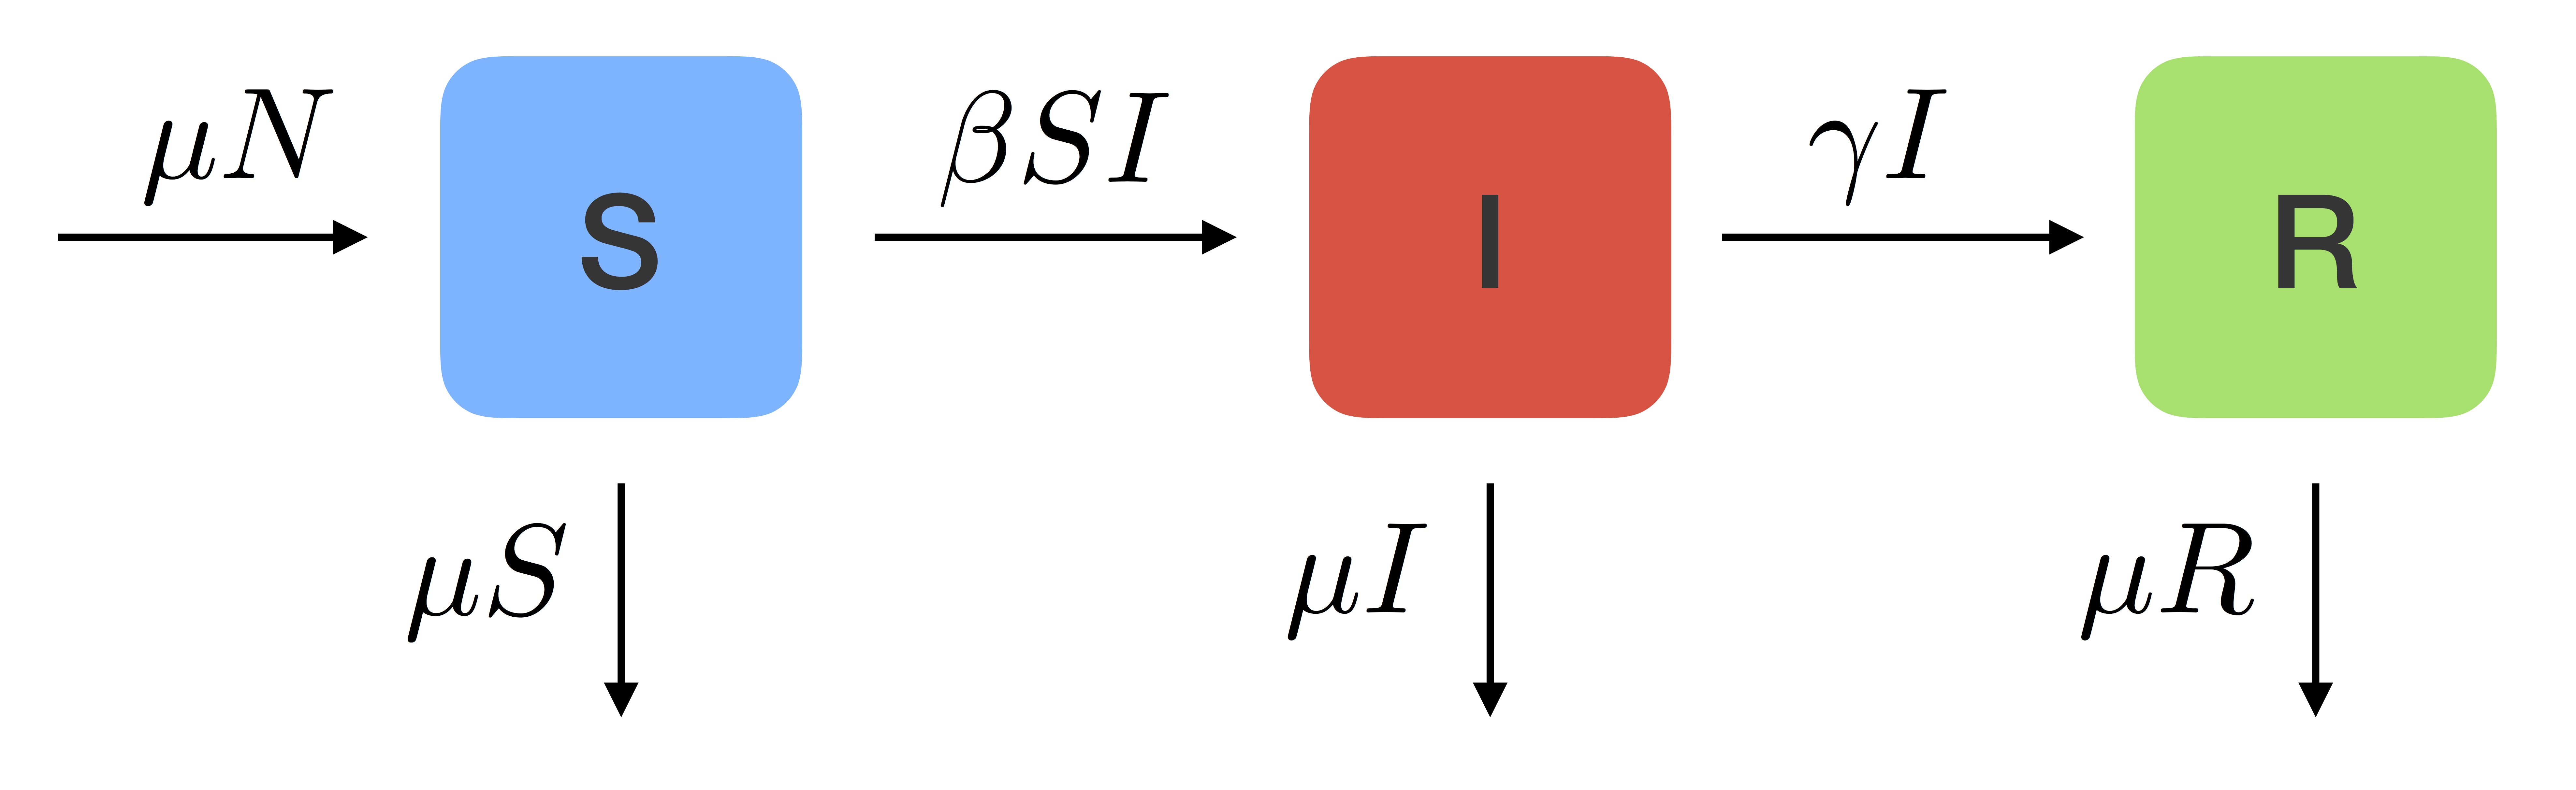
\includegraphics[width=0.6\linewidth]{flow.png}
    \caption{The SIR Model}
\end{figure}

The mathematical model that our group decided to use was the SIR model. We made a set of assumptions that most people on campus interact with about as many people we do, and that CSU students are only infected people associated with CSU and not around Fort Collins. We did this so that we could keep our population size down without it getting to complicated. 

SIR model is a model to simulate the process of an epidemic spread by vectors,which can infect susceptible individuals. In this model, we assume the total size ($N$) of population is constant, so birth and death are omitted in this model. And the total population is divided into three categories, $S$ (susceptible), $I$ (infectious), $R$ (removed) individuals.

\begin{equation}
    N=S+I+R  \label{A}
\end{equation}

In this model, we have two different processes. The first one is between S and I individuals. In our real world, the rate of infection is dynamic,because there are all kinds of elements to influence it,such as temperature, humidity, and air quality. However,for keep this model easy to simulate, we decided to use a positive constant parameter to be our transition rate $\beta$. It means the probability of getting infected when one susceptible and one infectious individual complete an interaction. The second is between I and R individuals. In our assumption, this disease becomes noninfectious. As time goes by, some patients will recover and will not be infected twice. And the rate of recovery is also a positive constant parameter, $\gamma$, which is less than $\beta$. In the case, which $\gamma > \beta$, the disease will not spread. Lastly, we assume one day to be our time unit. Under these assumptions, we have an SIR model which has the following set of ordinary differential equations \cite{hethcote2000mathematics}:

\begin{subequations}
    \label{eq:sys}
    \begin{align}
        \frac{dS}{dt} &= -\frac{\beta I S}{N}\, \label{eq:ds} \\
        \frac{dI}{dt} &= \frac{\beta I S}{N} - \gamma I\, \label{eq:di} \\
        \frac{dR}{dt} &= \gamma I\, \label{eq:dr}
    \end{align}
\end{subequations}
    
After established our SIR model for this simulation, our group wanted to find the appropriate parameters to put in our simulation. Because our goal is finding out how long a disease will spread across CSU, the disease must have large transition rate. If a disease need more than one year to infect all people, it’s not good for our model. As an university, every year, CSU has lots of freshman getting into the university and also big number of senior students, who leave out of CSU. This change cannot be ignored without invalidating our simulation.  We assume that this disease is not fatal, so no one will die due to the infection.

To simulate the SIR and SI models, we used Python. We built an ODE solver class which takes a system of differential equations (a list of functions) and an initial value. It is similar to scipy.integrate.solve\_ivp, but more limited, and we programmed it ourselves. The passed functions take a scalar time value and a vector. The vector contains the variables which the system of differential equations describe. For example, SIR has three functions, $\frac{dS}{dt}, \frac{dI}{dt}, \frac{dR}{dt}$. Then, the vector is those variables approximated given the initial value. The approximation is carried out by 4th order Runge-Kutta. With short simulations, we can afford to have small time steps. The, we can ignore explicit/implicit and stiff/nonstiff considerations.

Let
\begin{equation}
    \Fv(t) = 
    \left(
    \begin{matrix}
        S \\
        I \\
        R \\
    \end{matrix}
    \right)
\end{equation}

where S is the susceptible population, I is the infected population, and R is the recovered/removed population.

Then, let the following system of differential equations govern the populations, $\Fv$:

\begin{align*}
    \fv(t, S, I, R) &= 
    \left(
    \begin{matrix}
        dS/dt \\
        dI/dt \\
        dR/dt \\
    \end{matrix}
    \right) \\
    &= 
    \begin{pmatrix}
        -\frac{\beta I S}{N} \\
        \frac{\beta I S}{N} - \gamma I \\
        \gamma I
    \end{pmatrix}
\end{align*}

Given $\Fv_0 = \Fv(t_0) = (S_0, I_0, R_0)$ where $t_0=0$, Runge-Kutta's method allows us to simulate $\Fv$ with the following step function given some $h = \Delta t$ \cite{endre2003introduction}.

\begin{align}
    \Fv_{n+1} &= \Fv_n + \frac{1}{6}\left(\kv_1 + 2\kv_2 + 2\kv_3+\kv_4\right) \\
    t_{n+1} &= t_n+h
\end{align}
where
\begin{align}
    h &= \Delta t \\
    \kv_1 &= h \fv(t_n, \Fv_n) \\
    \kv_2 &= h \fv(t_n+\frac{h}{2}, \Fv_n + \frac{\kv_1}{2}) \\
    \kv_3 &= h \fv(t_n+\frac{h}{2}, \Fv_n + \frac{\kv_2}{2}) \\
    \kv_4 &= h \fv(t_n+h, \Fv_n+\kv_3) \\
\end{align}

By using very small $\Delta t$ and taking as many steps as needed, until $t_n$ reaches our desired time, we can approximate the evolution of our model over time.

For our experimentation, we used different parameters and fed them to our solver to run the simulation. The two parameters are $\beta$ and $\gamma$ (described above). Loosely, $\beta$ is the infection rate and $\gamma$ is the recovery rate. To find $\beta$, we collected our own data by approximating the number of people we would come in contact with over the course of 24 hours (Table \ref{tab:peopls}).

\begin{table}[H]
    \centering
    \begin{tabular}{c|c|c|c|c|c}
        Names & Lucas & Zhanhong & Sharon & Rachel & Total \\ \hline
        Day Sample &  Weekend & M/W/F & M/W/F & Tu/Th & \\ \hline
        Number of People & 8 & 5 & 10 & 19 & 42
    \end{tabular}
    \caption{Collected exposure data}
    \label{tab:peopls}
\end{table}

Using this data, we can construct the expected number of people to be infected after a 24 hour period:

\begin{equation}
    I = \text{Initial Infected} + \text{Infection Chance} \times \text{Total Exposed In 24 Hours}
\end{equation}

In our case, initial infected was us 4, and total exposed in 24 hours was 42.

Assuming this number of people will be infected, we use our SI model and simulate different $\beta$ values. We repeated this process with different betas until we were able to converge to to one which had that number of people infected after 24 hours. It might be possible to solve the problem analytically, but since it was nonlinear and simulations were cheap, we opted to go this route.


\begin{table}[H]
    \centering
    \begin{tabular}{c|ccccc}
        percent &  0\% &  25\% &  50\% &  75\% &  100\% \\ \hline
        $\beta$ & 0 & 1.61e-06 & 2.28e-06 & 2.73e-06 & 3.05e-06
        %\beta & 0 & 1.606308e-06 & 2.283956e-06 & 2.726045e-06 & 3.047978e-06
    \end{tabular}
    \caption{Found $\beta$ values for infection rate}
    \label{tab:betas}
\end{table}

We also investigated the SIR model. We used the 75\% beta value and varied $\gamma$, recover rate. We manually tried several different values to see the effects: 1, 0.1, 0.05, and 0.01.

\section{Results}
For an infection rate of 0\%, it does just what we’d expect. There were none that became infected, and the 4 initially infected (we), remained infected.

\begin{figure}[H]
    \centering
    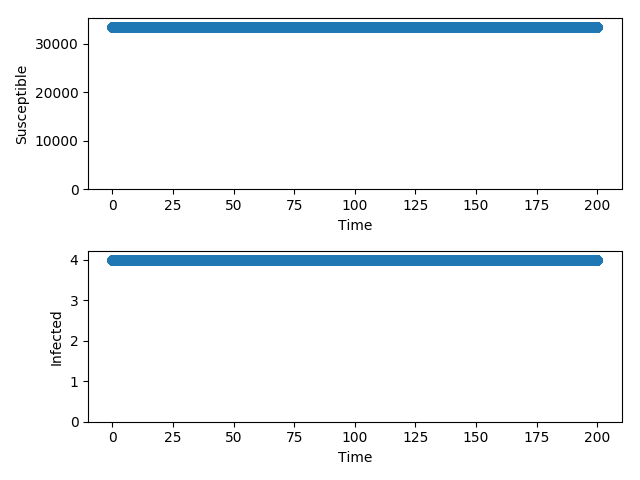
\includegraphics[width=0.6\linewidth]{0per.png}
    \caption{SI for 0\%}
\end{figure}

For an infection rate of 25\%, 50\% and 100\%, they look mostly the same, but the infection spread is slower for smaller infection rates.

\begin{figure}[H]
    \centering
    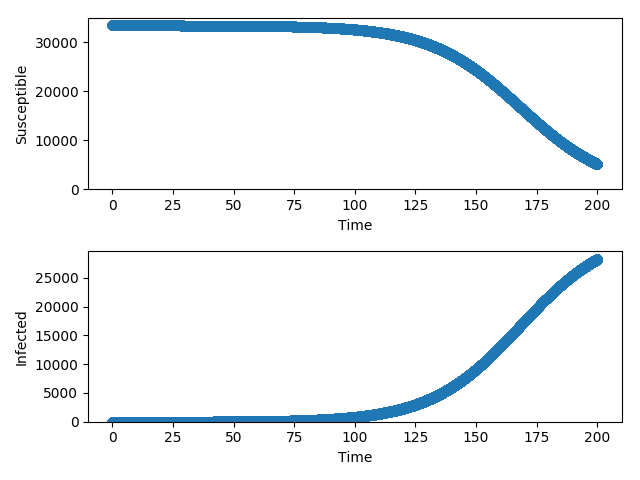
\includegraphics[width=0.6\linewidth]{25per.png}
    \caption{SI for 25\%}
\end{figure}

\begin{figure}[H]
    \centering
    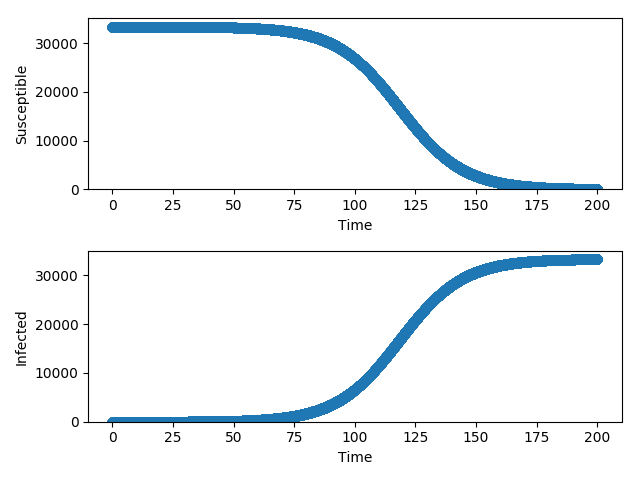
\includegraphics[width=0.6\linewidth]{50per.png}
    \caption{SI for 50\%}
\end{figure}

\begin{figure}[H]
    \centering
    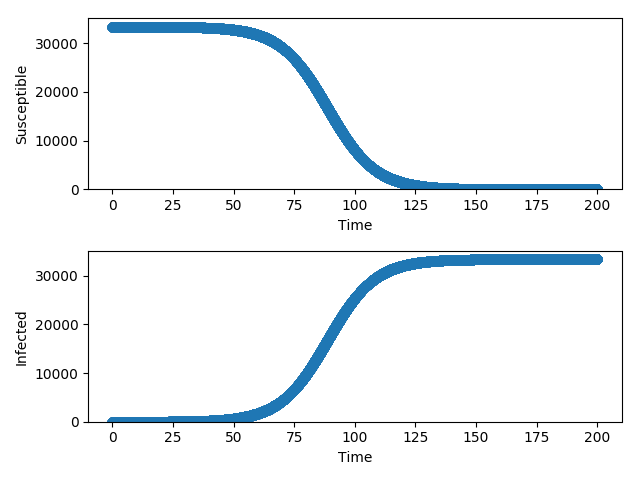
\includegraphics[width=0.6\linewidth]{100per.png}
    \caption{SI for 100\%}
\end{figure}

When we vary recover rate, we can see its effects on the infected population. The recovery rate removes those who have been infected for longer periods of time. As the disease spreads, more become infected, but then when less are being infected, those removed becomes more apparent, and infected begins to fall; hence, the hump.

For a slow recovery rate of 0.01, everyone gets infected since the infected population can’t be contained. Once everyone is infected, the drop becomes apparent.

\begin{figure}[H]
    \centering
    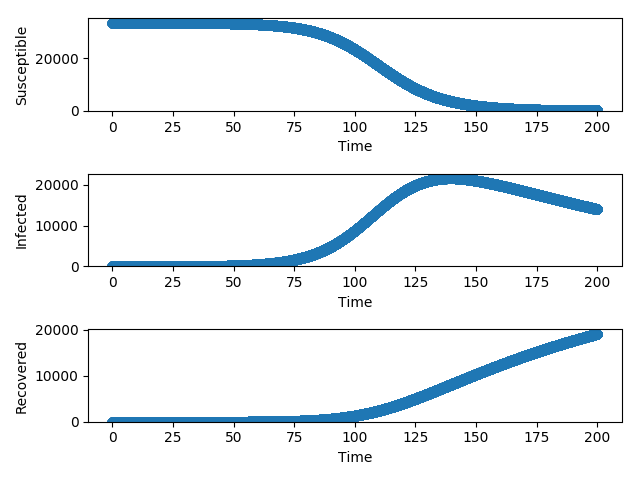
\includegraphics[width=0.6\linewidth]{g0p01.png}
    \caption{SIR model with $\gamma = 0.01$ for 75\% infection rate}
\end{figure}

For $\gamma = 0.05$, we see that it’s fast enough to fight the infected population. Infected grows rapidly, but eventually, the number recovering and the lesser amount susceptible causes infected to drop to zero. Then, the population stabilizes with few remaining uninfected.

\begin{figure}[H]
    \centering
    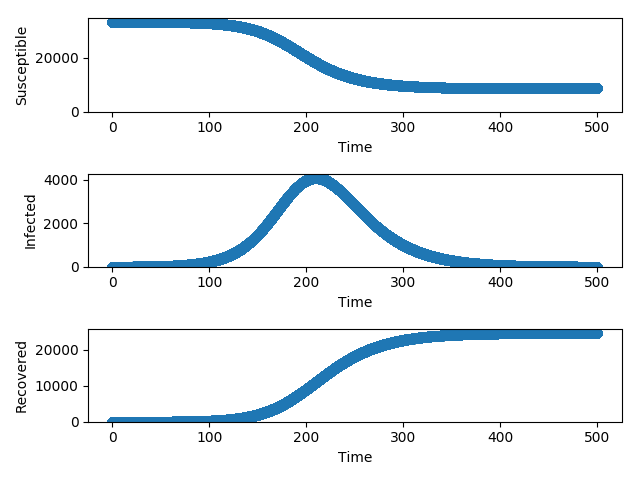
\includegraphics[width=0.6\linewidth]{g0p05.png}
    \caption{SIR model with $\gamma = 0.05$ for 75\% infection rate}
\end{figure}

When the recovery rate is moderately high, people stop being infected faster than they become infected. As a result, never more than 4 people become infected. However, notice that the hours it takes for the infected population to reach zero takes 200 hours (roughly 8 days). From the recovered graph, we can see roughly 40 people total were infected.

\begin{figure}[H]
    \centering
    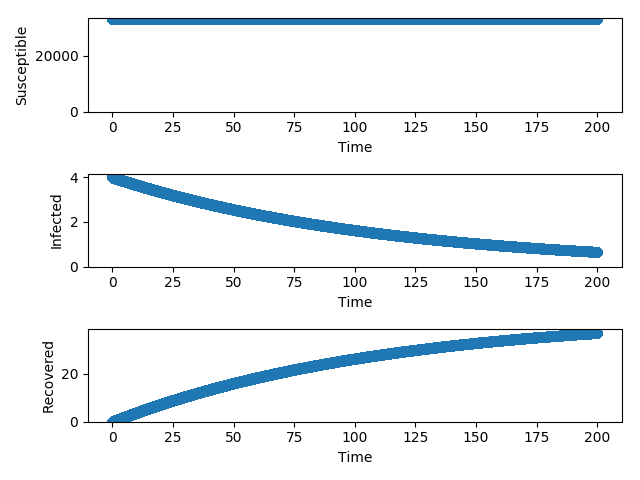
\includegraphics[width=0.6\linewidth]{g0p1.png}
    \caption{SIR model with $\gamma = 0.1$ for 75\% infection rate}
\end{figure}

When $\gamma$ is very large, 1.0, then the infected population drops to zero immediately, and no one else is infected. 

\begin{figure}[H]
    \centering
    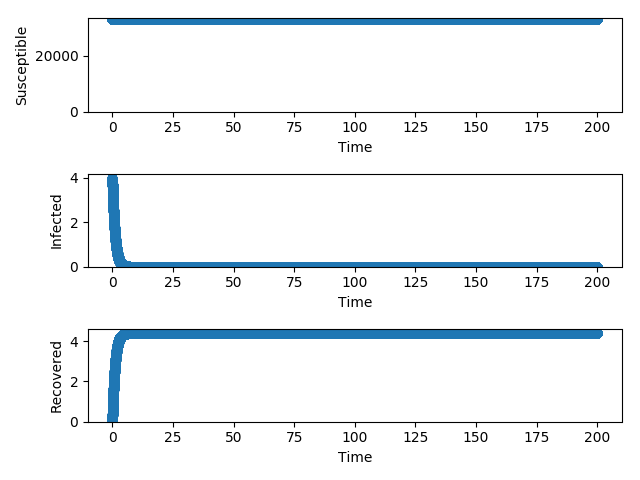
\includegraphics[width=0.6\linewidth]{g1p0.png}
    \caption{SIR model with $\gamma = 1.0$ for 75\% infection rate}
\end{figure}

\section{Future Work}
If our group was given another month or two to work on our project, we would of taken more time to collect real data. We would of gotten a larger sample size of CSU students and surveyed how many people a day they come into contact with and get a better average. We would really want our average to represent how many students are coming into contact with each other and what kind of contact. This would lead us into different ways of infection, like if students are greeting each other with a hug, handshake, just talking closely, etc. We could create different classifications for how the disease spreads to become more particular about how the disease spreads.

We could make assumptions about the disease and find a more realistic recovery rate, and we could probably add more components to the model, such as recovered becoming susceptible again.

\section{Conclusions}
After conducting our simulation, we found that ignoring the recovery, infection will spread more slowly under a lower infection rate. Then we added on the recovery rate. We found that with a very low recovery rate (0.01), people will not start to recover until everyone is infected. After that, we increased the recovery rate to median rate (0.05), we found that as our recovery rate increases, both of our infection and recovery number grow slower. It takes more time to get to the peak and also to start recover and it also faster to drop to the full recovery. When we had a high recovery rate (0.1), we found that no one will be infected anymore; people will start recovery before they get infected. The reason for this situation is that the two parameters cannot independent explain the two processes. Populations play a big role in the two change.


\section{Work Distribution}

\begin{itemize}
    \item Rachel Slark - created outline and started content in each section, wrote Motivation, future work
    \item Lucas Wilson - implemented SIR model
    \item Sharon Han - did research about SIR model contributing to introduction, wrote conclusion
    \item Zhanhong Luo -  wrote Data, Methods parts and part of introduction.
    \item All helped with final editing the report
\end{itemize}

\bibliography{main} 
\bibliographystyle{ieeetr}

\end{document}